\documentclass[aspectratio=169]{beamer}

% Packages
\usepackage{tikz}
\usepackage{graphicx}
\usepackage{hyperref}
\usepackage{xcolor}
\usepackage{fontspec}
\usepackage{booktabs}
\usepackage{amsmath}
\usepackage{array}

% Databricks Color Definitions
\definecolor{databricksBlue}{RGB}{41, 49, 66}
\definecolor{databricksRed}{RGB}{220, 53, 69}
\definecolor{databricksYellow}{RGB}{255, 193, 7}
\definecolor{databricksGreen}{RGB}{76, 175, 80}
\definecolor{databricksGray}{RGB}{128, 128, 128}
\definecolor{databricksLightGray}{RGB}{245, 245, 245}
\definecolor{databricksWhite}{RGB}{255, 255, 255}

% Beamer Theme Configuration
\usetheme{default}
\usecolortheme{default}

% Remove navigation symbols
\setbeamertemplate{navigation symbols}{}

% Set colors
\setbeamercolor{structure}{fg=databricksBlue}
\setbeamercolor{background canvas}{bg=databricksWhite}
\setbeamercolor{normal text}{fg=databricksBlue}
\setbeamercolor{frametitle}{fg=databricksWhite, bg=databricksBlue}
\setbeamercolor{title}{fg=databricksWhite}
\setbeamercolor{subtitle}{fg=databricksLightGray}
\setbeamercolor{author}{fg=databricksWhite}
\setbeamercolor{date}{fg=databricksWhite}
\setbeamercolor{institute}{fg=databricksLightGray}

% Frame title formatting
\setbeamertemplate{frametitle}{
    \nointerlineskip
    \begin{beamercolorbox}[wd=\paperwidth, ht=1.2cm, dp=0.3cm]{frametitle}
        \hspace*{0.5cm}\usebeamerfont{frametitle}\insertframetitle
    \end{beamercolorbox}
}

% Footline with three-part layout
\setbeamertemplate{footline}{
    \leavevmode%
    \hbox{%
        \begin{beamercolorbox}[wd=.33\paperwidth,ht=0.5cm,dp=0.2cm,left]{author in head/foot}%
            \usebeamerfont{author in head/foot}\hspace*{0.3cm}%
            \textcolor{databricksBlue}{\href{https://easy-ai-labs.lovable.app/}{Easy AI Labs}}
        \end{beamercolorbox}%
        \begin{beamercolorbox}[wd=.34\paperwidth,ht=0.5cm,dp=0.2cm,center]{title in head/foot}%
            \usebeamerfont{title in head/foot}%
            \textcolor{databricksBlue}{\href{https://www.linkedin.com/in/yashkavaiya}{Yash Kavaiya}}
        \end{beamercolorbox}%
        \begin{beamercolorbox}[wd=.33\paperwidth,ht=0.5cm,dp=0.2cm,right]{date in head/foot}%
            \usebeamerfont{date in head/foot}%
            \textcolor{databricksBlue}{\href{https://www.linkedin.com/company/genai-guru}{Gen AI Guru}}%
            \hspace*{0.5cm}%
            \textcolor{databricksGray}{\insertframenumber{}/\inserttotalframenumber}\hspace*{0.3cm}
        \end{beamercolorbox}%
    }%
    \vskip0pt%
}

% Title page template
\defbeamertemplate*{title page}{customized}[1][]
{
    \begin{tikzpicture}[remember picture, overlay]
        \fill[databricksBlue] (current page.north west) rectangle (current page.south east);
    \end{tikzpicture}
    \vfill
    \begin{center}
        {\Huge\textcolor{databricksWhite}{\textbf{\inserttitle}}\par}
        \vspace{0.5cm}
        {\large\textcolor{databricksLightGray}{\insertsubtitle}\par}
        \vspace{1cm}
        {\textcolor{databricksYellow}{\insertauthor}\par}
        \vspace{0.3cm}
        {\small\textcolor{databricksLightGray}{\insertinstitute}\par}
        \vspace{0.5cm}
        {\small\textcolor{databricksGray}{\insertdate}\par}
    \end{center}
    \vfill
}

% Custom itemize
\setbeamertemplate{itemize item}{\textcolor{databricksBlue}{$\bullet$}}
\setbeamertemplate{itemize subitem}{\textcolor{databricksRed}{$\triangleright$}}
\setbeamertemplate{itemize subsubitem}{\textcolor{databricksGreen}{$\circ$}}

% Title information
\title{Lakehouse Architecture Basics}
\subtitle{Day 3 - Databricks 14-Day AI Challenge}
\author{Yash Kavaiya}
\institute{Gen AI Guru | Easy AI Labs}
\date{\today}

\begin{document}

% Title Slide
\frame{\titlepage}

% Outline Slide
\begin{frame}{Agenda}
    \begin{itemize}
        \item \textcolor{databricksBlue}{\textbf{Data Architectures Evolution}} - From Warehouses to Lakehouse
        \item \textcolor{databricksBlue}{\textbf{What is a Data Lakehouse?}} - Combining the best of both worlds
        \item \textcolor{databricksBlue}{\textbf{Delta Lake}} - The foundation of Lakehouse
        \item \textcolor{databricksBlue}{\textbf{Lakehouse Components}} - Complete architecture overview
        \item \textcolor{databricksBlue}{\textbf{ACID Transactions}} - Ensuring data reliability
        \item \textcolor{databricksBlue}{\textbf{Medallion Architecture}} - Bronze, Silver, Gold layers
    \end{itemize}
\end{frame}

% Section: Data Architectures Evolution
\begin{frame}{Data Architectures Evolution}
    \begin{center}
        \textcolor{databricksBlue}{\Large\textbf{The Journey to Modern Data Architecture}}
    \end{center}
    \vspace{0.5cm}
    \begin{columns}[T]
        \begin{column}{0.45\textwidth}
            \textcolor{databricksRed}{\textbf{Phase 1: Data Warehouses (1980s-2000s)}}
            \begin{itemize}
                \item Structured data only
                \item ACID transactions
                \item SQL-based querying
                \item High cost per TB
            \end{itemize}
        \end{column}
        \begin{column}{0.45\textwidth}
            \textcolor{databricksGreen}{\textbf{Phase 2: Data Lakes (2010s)}}
            \begin{itemize}
                \item All data types
                \item Schema-on-read
                \item Low cost storage
                \item Poor reliability
            \end{itemize}
        \end{column}
    \end{columns}
\end{frame}

% Data Warehouse Details
\begin{frame}{Phase 1: Data Warehouses}
    \begin{center}
        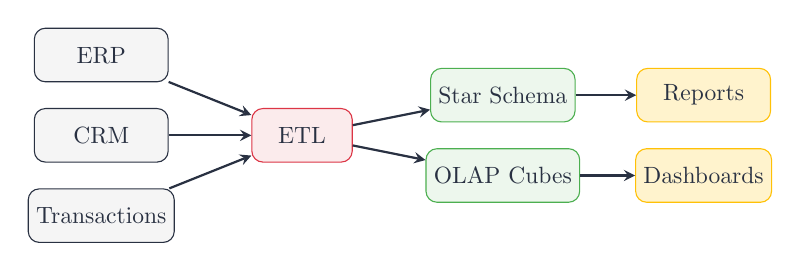
\begin{tikzpicture}[scale=0.85, transform shape]
            % Styles
            \tikzstyle{source} = [rectangle, draw=databricksBlue, fill=databricksLightGray, text=databricksBlue, minimum width=2cm, minimum height=0.8cm, rounded corners]
            \tikzstyle{process} = [rectangle, draw=databricksRed, fill=databricksRed!10, text=databricksBlue, minimum width=1.5cm, minimum height=0.8cm, rounded corners]
            \tikzstyle{warehouse} = [rectangle, draw=databricksGreen, fill=databricksGreen!10, text=databricksBlue, minimum width=2cm, minimum height=0.8cm, rounded corners]
            \tikzstyle{bi} = [rectangle, draw=databricksYellow, fill=databricksYellow!20, text=databricksBlue, minimum width=2cm, minimum height=0.8cm, rounded corners]
            \tikzstyle{arrow} = [->, >=stealth, thick, databricksBlue]
            
            % Nodes - explicit coordinates
            \node[source] (erp) at (0, 1.2) {ERP};
            \node[source] (crm) at (0, 0) {CRM};
            \node[source] (txn) at (0, -1.2) {Transactions};
            
            \node[process] (etl) at (3, 0) {ETL};
            
            \node[warehouse] (schema) at (6, 0.6) {Star Schema};
            \node[warehouse] (olap) at (6, -0.6) {OLAP Cubes};
            
            \node[bi] (reports) at (9, 0.6) {Reports};
            \node[bi] (dash) at (9, -0.6) {Dashboards};
            
            % Arrows
            \draw[arrow] (erp) -- (etl);
            \draw[arrow] (crm) -- (etl);
            \draw[arrow] (txn) -- (etl);
            \draw[arrow] (etl) -- (schema);
            \draw[arrow] (etl) -- (olap);
            \draw[arrow] (schema) -- (reports);
            \draw[arrow] (olap) -- (dash);
        \end{tikzpicture}
    \end{center}
    \vspace{0.3cm}
    \textcolor{databricksRed}{\textbf{Limitation:}} Not suitable for unstructured data (images, logs, JSON)
\end{frame}

% Data Lake Details
\begin{frame}{Phase 2: Data Lakes}
    \begin{center}
        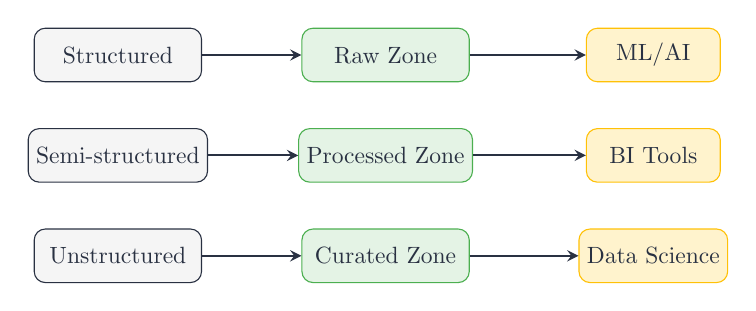
\begin{tikzpicture}[scale=0.85, transform shape]
            % Styles
            \tikzstyle{source} = [rectangle, draw=databricksBlue, fill=databricksLightGray, text=databricksBlue, minimum width=2.5cm, minimum height=0.8cm, rounded corners]
            \tikzstyle{lake} = [rectangle, draw=databricksGreen, fill=databricksGreen!15, text=databricksBlue, minimum width=2.5cm, minimum height=0.8cm, rounded corners]
            \tikzstyle{consumer} = [rectangle, draw=databricksYellow, fill=databricksYellow!20, text=databricksBlue, minimum width=2cm, minimum height=0.8cm, rounded corners]
            \tikzstyle{arrow} = [->, >=stealth, thick, databricksBlue]
            
            % Source Nodes - explicit coordinates
            \node[source] (str) at (0, 1.5) {Structured};
            \node[source] (semi) at (0, 0) {Semi-structured};
            \node[source] (un) at (0, -1.5) {Unstructured};
            
            % Lake Nodes
            \node[lake] (raw) at (4, 1.5) {Raw Zone};
            \node[lake] (proc) at (4, 0) {Processed Zone};
            \node[lake] (cur) at (4, -1.5) {Curated Zone};
            
            % Consumer Nodes
            \node[consumer] (ml) at (8, 1.5) {ML/AI};
            \node[consumer] (bi) at (8, 0) {BI Tools};
            \node[consumer] (ds) at (8, -1.5) {Data Science};
            
            % Arrows
            \draw[arrow] (str) -- (raw);
            \draw[arrow] (semi) -- (proc);
            \draw[arrow] (un) -- (cur);
            \draw[arrow] (raw) -- (ml);
            \draw[arrow] (proc) -- (bi);
            \draw[arrow] (cur) -- (ds);
        \end{tikzpicture}
    \end{center}
    \vspace{0.3cm}
    \textcolor{databricksRed}{\textbf{Problem:}} No ACID transactions $\rightarrow$ \textbf{``Data Swamps''}
\end{frame}

% Two-Tier Problem
\begin{frame}{The Two-Tier Architecture Problem}
    \begin{columns}[T]
        \begin{column}{0.5\textwidth}
            \begin{center}
                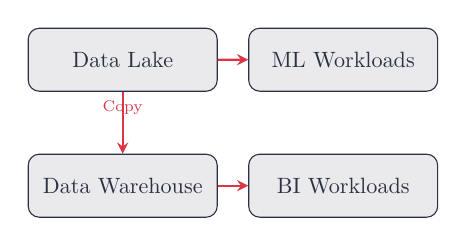
\begin{tikzpicture}[scale=0.8, transform shape]
                    \tikzstyle{box} = [rectangle, draw=databricksBlue, fill=databricksBlue!10, text=databricksBlue, minimum width=3cm, minimum height=1cm, rounded corners]
                    \tikzstyle{arrow} = [->, >=stealth, thick, databricksRed]
                    
                    \node[box] (dl) at (0, 2) {Data Lake};
                    \node[box] (dw) at (0, 0) {Data Warehouse};
                    \node[box] (ml) at (3.5, 2) {ML Workloads};
                    \node[box] (bi) at (3.5, 0) {BI Workloads};
                    
                    \draw[arrow] (dl) -- node[above, font=\scriptsize] {Copy} (dw);
                    \draw[arrow] (dl) -- (ml);
                    \draw[arrow] (dw) -- (bi);
                \end{tikzpicture}
            \end{center}
        \end{column}
        \begin{column}{0.45\textwidth}
            \textcolor{databricksRed}{\textbf{Problems:}}
            \begin{itemize}
                \item \textcolor{databricksBlue}{$\bullet$} Data duplication
                \item \textcolor{databricksBlue}{$\bullet$} Stale data
                \item \textcolor{databricksBlue}{$\bullet$} Complex pipelines
                \item \textcolor{databricksBlue}{$\bullet$} High costs
                \item \textcolor{databricksBlue}{$\bullet$} Governance challenges
            \end{itemize}
        \end{column}
    \end{columns}
\end{frame}

% What is Lakehouse
\begin{frame}{What is a Data Lakehouse?}
    \begin{center}
        \textcolor{databricksBlue}{\Large\textbf{The Best of Both Worlds}}
        \vspace{0.5cm}
        
        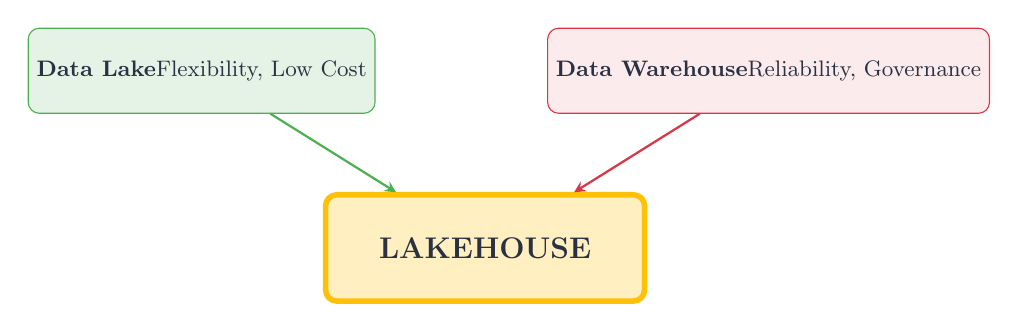
\begin{tikzpicture}[scale=0.9, transform shape]
            \tikzstyle{lakebox} = [rectangle, draw=databricksGreen, fill=databricksGreen!15, text=databricksBlue, minimum width=4cm, minimum height=1.2cm, rounded corners, font=\small]
            \tikzstyle{whbox} = [rectangle, draw=databricksRed, fill=databricksRed!10, text=databricksBlue, minimum width=4cm, minimum height=1.2cm, rounded corners, font=\small]
            \tikzstyle{lhbox} = [rectangle, draw=databricksYellow, fill=databricksYellow!25, text=databricksBlue, minimum width=4.5cm, minimum height=1.5cm, rounded corners, font=\large, line width=2pt]
            
            \node[lakebox] (lake) at (-4, 0) {\textbf{Data Lake}\\Flexibility, Low Cost};
            \node[whbox] (wh) at (4, 0) {\textbf{Data Warehouse}\\Reliability, Governance};
            \node[lhbox] (lh) at (0, -2.5) {\textbf{LAKEHOUSE}};
            
            \draw[->, >=stealth, thick, databricksGreen] (lake) -- (lh);
            \draw[->, >=stealth, thick, databricksRed] (wh) -- (lh);
        \end{tikzpicture}
    \end{center}
\end{frame}

% Key Lakehouse Principles
\begin{frame}{Key Lakehouse Principles}
    \begin{center}
        \small
        \begin{tabular}{>{\raggedright\arraybackslash}p{3cm} >{\raggedright\arraybackslash}p{4.5cm} >{\raggedright\arraybackslash}p{4cm}}
            \toprule
            \textcolor{databricksBlue}{\textbf{Principle}} & \textcolor{databricksBlue}{\textbf{Description}} & \textcolor{databricksBlue}{\textbf{Benefit}} \\
            \midrule
            \textcolor{databricksRed}{Open Formats} & Data in Parquet, Delta & No vendor lock-in \\
            \textcolor{databricksRed}{ACID Transactions} & Reliable updates & Data consistency \\
            \textcolor{databricksRed}{Schema Enforcement} & Data quality at write & Prevent bad data \\
            \textcolor{databricksRed}{Time Travel} & Access previous versions & Auditing, rollback \\
            \textcolor{databricksRed}{Unified Access} & Same data for all & No data silos \\
            \textcolor{databricksRed}{Direct Access} & Query in place & No copying needed \\
            \bottomrule
        \end{tabular}
    \end{center}
\end{frame}

% Delta Lake Introduction
\begin{frame}{Delta Lake: The Foundation}
    \begin{columns}[T]
        \begin{column}{0.55\textwidth}
            \textcolor{databricksBlue}{\textbf{What is Delta Lake?}}
            \vspace{0.3cm}
            
            An \textcolor{databricksRed}{\textbf{open-source storage layer}} that brings reliability to Data Lakes.
            \vspace{0.5cm}
            
            \textcolor{databricksGreen}{\textbf{How it works:}}
            \begin{itemize}
                \item Stores data as \textbf{Parquet files}
                \item Adds a \textbf{transaction log}
                \item Enables ACID on object storage
            \end{itemize}
        \end{column}
        \begin{column}{0.4\textwidth}
            \textcolor{databricksBlue}{\textbf{Table Structure:}}
            \vspace{0.2cm}
            
            \ttfamily\footnotesize
            \textcolor{databricksGray}{delta\_table/}\\
            \textcolor{databricksRed}{+-- \_delta\_log/}\\
            \textcolor{databricksGray}{\textbar\hspace{0.3cm}+-- 000...00.json}\\
            \textcolor{databricksGray}{\textbar\hspace{0.3cm}+-- 000...01.json}\\
            \textcolor{databricksGray}{\textbar\hspace{0.3cm}+-- 000...02.json}\\
            \textcolor{databricksGreen}{+-- part-00000.parquet}\\
            \textcolor{databricksGreen}{+-- part-00001.parquet}\\
            \textcolor{databricksGreen}{+-- part-00002.parquet}
        \end{column}
    \end{columns}
\end{frame}

% Delta Lake Features
\begin{frame}{Delta Lake Features}
    \begin{center}
        \small
        \begin{tabular}{>{\raggedright\arraybackslash}p{3cm} >{\raggedright\arraybackslash}p{4cm} >{\raggedright\arraybackslash}p{4.5cm}}
            \toprule
            \textcolor{databricksBlue}{\textbf{Feature}} & \textcolor{databricksBlue}{\textbf{Description}} & \textcolor{databricksBlue}{\textbf{Example}} \\
            \midrule
            \textcolor{databricksGreen}{ACID Transactions} & Atomic, reliable operations & Multiple concurrent writers \\
            \textcolor{databricksGreen}{Time Travel} & Query historical data & \texttt{VERSION AS OF 5} \\
            \textcolor{databricksGreen}{Schema Evolution} & Add columns safely & \texttt{ALTER TABLE ADD COL} \\
            \textcolor{databricksGreen}{Schema Enforcement} & Reject invalid data & Wrong types fail \\
            \textcolor{databricksGreen}{Audit History} & Track all changes & \texttt{DESCRIBE HISTORY} \\
            \textcolor{databricksGreen}{MERGE (Upserts)} & Update/Insert combined & CDC processing \\
            \bottomrule
        \end{tabular}
    \end{center}
\end{frame}

% Time Travel Example
\begin{frame}[fragile]{Time Travel in Action}
    \begin{center}
        \textcolor{databricksBlue}{\large\textbf{Query Any Version of Your Data}}
    \end{center}
    \vspace{0.3cm}
    
    \begin{columns}[T]
        \begin{column}{0.48\textwidth}
            \textcolor{databricksGreen}{\textbf{Query by Version:}}
            \vspace{0.2cm}
            
            \ttfamily\small
            \textcolor{databricksGray}{-- Current version}\\
            SELECT * FROM sales;\\
            \vspace{0.3cm}
            \textcolor{databricksGray}{-- Specific version}\\
            SELECT * FROM sales\\
            \textcolor{databricksRed}{VERSION AS OF 5};
        \end{column}
        \begin{column}{0.48\textwidth}
            \textcolor{databricksGreen}{\textbf{Query by Timestamp:}}
            \vspace{0.2cm}
            
            \ttfamily\small
            \textcolor{databricksGray}{-- Point in time}\\
            SELECT * FROM sales\\
            \textcolor{databricksRed}{TIMESTAMP AS OF}\\
            \textcolor{databricksRed}{'2024-01-01'};\\
            \vspace{0.3cm}
            \textcolor{databricksGray}{-- Restore data}\\
            RESTORE TABLE sales\\
            \textcolor{databricksRed}{TO VERSION AS OF 5};
        \end{column}
    \end{columns}
\end{frame}

% Lakehouse Architecture Components
\begin{frame}{Complete Lakehouse Architecture}
    \begin{center}
        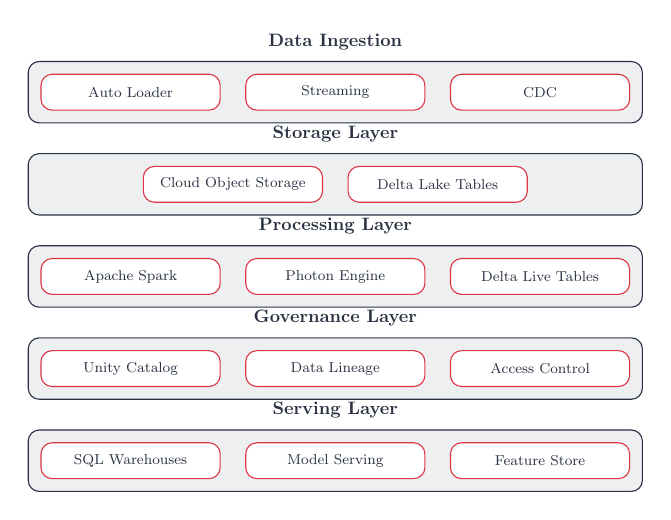
\begin{tikzpicture}[scale=0.65, transform shape]
            % Styles
            \tikzstyle{layer} = [rectangle, draw=databricksBlue, fill=databricksBlue!8, text=databricksBlue, minimum width=12cm, minimum height=1.2cm, rounded corners]
            \tikzstyle{component} = [rectangle, draw=databricksRed, fill=databricksWhite, text=databricksBlue, minimum width=3.5cm, minimum height=0.7cm, rounded corners, font=\footnotesize]
            
            % Layers
            \node[layer] (ing) at (0, 4) {};
            \node[above=0.1cm] at (ing.north) {\textcolor{databricksBlue}{\textbf{Data Ingestion}}};
            \node[component] at (-4, 4) {Auto Loader};
            \node[component] at (0, 4) {Streaming};
            \node[component] at (4, 4) {CDC};
            
            \node[layer] (stor) at (0, 2.2) {};
            \node[above=0.1cm] at (stor.north) {\textcolor{databricksBlue}{\textbf{Storage Layer}}};
            \node[component] at (-2, 2.2) {Cloud Object Storage};
            \node[component] at (2, 2.2) {Delta Lake Tables};
            
            \node[layer] (proc) at (0, 0.4) {};
            \node[above=0.1cm] at (proc.north) {\textcolor{databricksBlue}{\textbf{Processing Layer}}};
            \node[component] at (-4, 0.4) {Apache Spark};
            \node[component] at (0, 0.4) {Photon Engine};
            \node[component] at (4, 0.4) {Delta Live Tables};
            
            \node[layer] (gov) at (0, -1.4) {};
            \node[above=0.1cm] at (gov.north) {\textcolor{databricksBlue}{\textbf{Governance Layer}}};
            \node[component] at (-4, -1.4) {Unity Catalog};
            \node[component] at (0, -1.4) {Data Lineage};
            \node[component] at (4, -1.4) {Access Control};
            
            \node[layer] (serv) at (0, -3.2) {};
            \node[above=0.1cm] at (serv.north) {\textcolor{databricksBlue}{\textbf{Serving Layer}}};
            \node[component] at (-4, -3.2) {SQL Warehouses};
            \node[component] at (0, -3.2) {Model Serving};
            \node[component] at (4, -3.2) {Feature Store};
        \end{tikzpicture}
    \end{center}
\end{frame}

% Data Ingestion Layer
\begin{frame}{Data Ingestion Layer}
    \begin{columns}[T]
        \begin{column}{0.32\textwidth}
            \begin{center}
                \textcolor{databricksRed}{\textbf{Auto Loader}}
            \end{center}
            \begin{itemize}
                \item[\textcolor{databricksBlue}{$\bullet$}] Incremental file ingestion
                \item[\textcolor{databricksBlue}{$\bullet$}] Schema inference
                \item[\textcolor{databricksBlue}{$\bullet$}] Exactly-once semantics
            \end{itemize}
        \end{column}
        \begin{column}{0.32\textwidth}
            \begin{center}
                \textcolor{databricksGreen}{\textbf{Streaming}}
            \end{center}
            \begin{itemize}
                \item[\textcolor{databricksBlue}{$\bullet$}] Kafka integration
                \item[\textcolor{databricksBlue}{$\bullet$}] Event Hubs
                \item[\textcolor{databricksBlue}{$\bullet$}] Kinesis support
            \end{itemize}
        \end{column}
        \begin{column}{0.32\textwidth}
            \begin{center}
                \textcolor{databricksYellow}{\textbf{CDC}}
            \end{center}
            \begin{itemize}
                \item[\textcolor{databricksBlue}{$\bullet$}] Database changes
                \item[\textcolor{databricksBlue}{$\bullet$}] Real-time sync
                \item[\textcolor{databricksBlue}{$\bullet$}] MERGE operations
            \end{itemize}
        \end{column}
    \end{columns}
\end{frame}

% Processing and Governance
\begin{frame}{Processing \& Governance Layers}
    \begin{columns}[T]
        \begin{column}{0.48\textwidth}
            \textcolor{databricksRed}{\textbf{Processing Layer}}
            \vspace{0.3cm}
            \begin{itemize}
                \item \textcolor{databricksBlue}{\textbf{Apache Spark:}} Core engine
                \item \textcolor{databricksBlue}{\textbf{Photon Engine:}} C++ vectorized\\
                \hspace{0.5cm}\textcolor{databricksGreen}{(2-8x faster)}
                \item \textcolor{databricksBlue}{\textbf{Delta Live Tables:}} Declarative ETL
            \end{itemize}
        \end{column}
        \begin{column}{0.48\textwidth}
            \textcolor{databricksGreen}{\textbf{Governance Layer}}
            \vspace{0.3cm}
            \begin{itemize}
                \item \textcolor{databricksBlue}{\textbf{Unity Catalog:}} Centralized governance
                \item \textcolor{databricksBlue}{\textbf{Data Lineage:}} Track data flow
                \item \textcolor{databricksBlue}{\textbf{Access Control:}} Row/column security
            \end{itemize}
        \end{column}
    \end{columns}
\end{frame}

% ACID Transactions
\begin{frame}{ACID Transactions in Lakehouse}
    \begin{center}
        \textcolor{databricksBlue}{\Large\textbf{Ensuring Data Reliability}}
    \end{center}
    \vspace{0.3cm}
    
    \begin{center}
        \small
        \begin{tabular}{>{\raggedright\arraybackslash}p{2.5cm} >{\raggedright\arraybackslash}p{4cm} >{\raggedright\arraybackslash}p{5cm}}
            \toprule
            \textcolor{databricksBlue}{\textbf{Property}} & \textcolor{databricksBlue}{\textbf{Definition}} & \textcolor{databricksBlue}{\textbf{Example}} \\
            \midrule
            \textcolor{databricksRed}{\textbf{Atomicity}} & All succeed or all fail & Debit AND credit both happen \\
            \textcolor{databricksGreen}{\textbf{Consistency}} & Data always valid & Balance never negative \\
            \textcolor{databricksYellow}{\textbf{Isolation}} & No interference & Two concurrent updates \\
            \textcolor{databricksBlue}{\textbf{Durability}} & Survives failures & Power outage safe \\
            \bottomrule
        \end{tabular}
    \end{center}
\end{frame}

% How Delta Lake Achieves ACID
\begin{frame}{How Delta Lake Achieves ACID}
    \begin{columns}[T]
        \begin{column}{0.48\textwidth}
            \textcolor{databricksRed}{\textbf{1. Optimistic Concurrency}}
            \begin{itemize}
                \item[\textcolor{databricksBlue}{$\bullet$}] Writers don't block
                \item[\textcolor{databricksBlue}{$\bullet$}] Conflicts at commit
                \item[\textcolor{databricksBlue}{$\bullet$}] Automatic retry
            \end{itemize}
            \vspace{0.5cm}
            
            \textcolor{databricksGreen}{\textbf{2. Write-Ahead Log}}
            \begin{itemize}
                \item[\textcolor{databricksBlue}{$\bullet$}] Log before data
                \item[\textcolor{databricksBlue}{$\bullet$}] Enables recovery
            \end{itemize}
        \end{column}
        \begin{column}{0.48\textwidth}
            \textcolor{databricksYellow}{\textbf{3. Atomic Commits}}
            \begin{itemize}
                \item[\textcolor{databricksBlue}{$\bullet$}] New log entry = complete
                \item[\textcolor{databricksBlue}{$\bullet$}] Incomplete writes ignored
            \end{itemize}
            \vspace{0.5cm}
            
            \begin{center}
                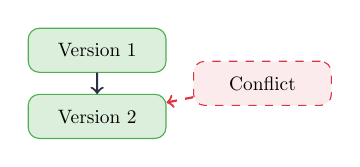
\begin{tikzpicture}[scale=0.7, transform shape]
                    \node[rectangle, draw=databricksGreen, fill=databricksGreen!20, minimum width=2.5cm, minimum height=0.8cm, rounded corners] (v1) at (0, 0) {Version 1};
                    \node[rectangle, draw=databricksGreen, fill=databricksGreen!20, minimum width=2.5cm, minimum height=0.8cm, rounded corners] (v2) at (0, -1.2) {Version 2};
                    \node[rectangle, draw=databricksRed, fill=databricksRed!10, minimum width=2.5cm, minimum height=0.8cm, rounded corners, dashed] (conflict) at (3, -0.6) {Conflict};
                    
                    \draw[->, thick, databricksBlue] (v1) -- (v2);
                    \draw[->, thick, databricksRed, dashed] (conflict) -- (v2);
                \end{tikzpicture}
            \end{center}
        \end{column}
    \end{columns}
\end{frame}

% Medallion Architecture
\begin{frame}{Medallion Architecture}
    \begin{center}
        \textcolor{databricksBlue}{\Large\textbf{Bronze $\rightarrow$ Silver $\rightarrow$ Gold}}
    \end{center}
    \vspace{0.3cm}
    
    \begin{center}
        
\begin{tikzpicture}[scale=0.85, transform shape]
            % Styles
            \tikzstyle{medal} = [rectangle, minimum width=3cm, minimum height=1.5cm, rounded corners=0.3cm, text=white, font=\bfseries]
            \tikzstyle{arrow} = [->, >=stealth, line width=2pt, databricksBlue]
            
            % Nodes
            \node[medal, fill={rgb:red,205;green,127;blue,50}] (bronze) at (0, 0) {\Large Bronze};
            \node[medal, fill={rgb:red,192;green,192;blue,192}] (silver) at (4.5, 0) {\Large Silver};
            \node[medal, fill={rgb:red,255;green,215;blue,0}, text=databricksBlue] (gold) at (9, 0) {\Large Gold};
            
            % Labels
            \node[below=0.3cm, text=databricksBlue, font=\small] at (bronze) {Raw Data};
            \node[below=0.3cm, text=databricksBlue, font=\small] at (silver) {Cleansed};
            \node[below=0.3cm, text=databricksBlue, font=\small] at (gold) {Curated};
            
            % Arrows
            \draw[arrow] (bronze) -- (silver);
            \draw[arrow] (silver) -- (gold);
        \end{tikzpicture}
    \end{center}
\end{frame}

% Bronze Layer
\begin{frame}{Bronze Layer - Raw Data}
    \begin{columns}[T]
        \begin{column}{0.48\textwidth}
            \textcolor{databricksBlue}{\textbf{Characteristics:}}
            \begin{itemize}
                \item[\textcolor{databricksRed}{$\triangleright$}] Raw data ``as-is'' from source
                \item[\textcolor{databricksRed}{$\triangleright$}] No transformations
                \item[\textcolor{databricksRed}{$\triangleright$}] Append-only writes
                \item[\textcolor{databricksRed}{$\triangleright$}] Full history preserved
                \item[\textcolor{databricksRed}{$\triangleright$}] Schema-on-read
            \end{itemize}
        \end{column}
        \begin{column}{0.48\textwidth}
            \textcolor{databricksGreen}{\textbf{Example:}}
            \begin{itemize}
                \item[\textcolor{databricksBlue}{$\bullet$}] Raw JSON from IoT sensors
                \item[\textcolor{databricksBlue}{$\bullet$}] CSV files from vendors
                \item[\textcolor{databricksBlue}{$\bullet$}] API response dumps
            \end{itemize}
            \vspace{0.5cm}
            
            \textcolor{databricksYellow}{\textbf{Quality:}} Low - may have errors, duplicates
        \end{column}
    \end{columns}
\end{frame}

% Silver Layer
\begin{frame}{Silver Layer - Cleansed Data}
    \begin{columns}[T]
        \begin{column}{0.48\textwidth}
            \textcolor{databricksBlue}{\textbf{Characteristics:}}
            \begin{itemize}
                \item[\textcolor{databricksRed}{$\triangleright$}] Cleaned and validated
                \item[\textcolor{databricksRed}{$\triangleright$}] Deduplication applied
                \item[\textcolor{databricksRed}{$\triangleright$}] Data types enforced
                \item[\textcolor{databricksRed}{$\triangleright$}] Joined with reference data
                \item[\textcolor{databricksRed}{$\triangleright$}] Schema enforced
            \end{itemize}
        \end{column}
        \begin{column}{0.48\textwidth}
            \textcolor{databricksGreen}{\textbf{Example:}}
            \begin{itemize}
                \item[\textcolor{databricksBlue}{$\bullet$}] Parsed sensor readings
                \item[\textcolor{databricksBlue}{$\bullet$}] Typed and validated
                \item[\textcolor{databricksBlue}{$\bullet$}] Deduplicated records
            \end{itemize}
            \vspace{0.5cm}
            
            \textcolor{databricksYellow}{\textbf{Quality:}} Medium - business rules applied
        \end{column}
    \end{columns}
\end{frame}

% Gold Layer
\begin{frame}{Gold Layer - Business Ready}
    \begin{columns}[T]
        \begin{column}{0.48\textwidth}
            \textcolor{databricksBlue}{\textbf{Characteristics:}}
            \begin{itemize}
                \item[\textcolor{databricksRed}{$\triangleright$}] Business-level aggregations
                \item[\textcolor{databricksRed}{$\triangleright$}] Denormalized for performance
                \item[\textcolor{databricksRed}{$\triangleright$}] Optimized for use cases
                \item[\textcolor{databricksRed}{$\triangleright$}] Multiple tables per domain
            \end{itemize}
        \end{column}
        \begin{column}{0.48\textwidth}
            \textcolor{databricksGreen}{\textbf{Example:}}
            \begin{itemize}
                \item[\textcolor{databricksBlue}{$\bullet$}] Hourly averages by location
                \item[\textcolor{databricksBlue}{$\bullet$}] Feature tables for ML
                \item[\textcolor{databricksBlue}{$\bullet$}] KPI dashboards
            \end{itemize}
            \vspace{0.5cm}
            
            \textcolor{databricksYellow}{\textbf{Quality:}} High - analytics ready
        \end{column}
    \end{columns}
\end{frame}

% Summary
\begin{frame}{Key Takeaways}
    \begin{itemize}
        \item \textcolor{databricksBlue}{\textbf{Lakehouse}} = Data Lake flexibility + Data Warehouse reliability
        \vspace{0.3cm}
        \item \textcolor{databricksRed}{\textbf{Delta Lake}} provides ACID transactions on object storage
        \vspace{0.3cm}
        \item \textcolor{databricksGreen}{\textbf{Time Travel}} enables auditing and rollback capabilities
        \vspace{0.3cm}
        \item \textcolor{databricksYellow}{\textbf{Medallion Architecture:}} Bronze $\rightarrow$ Silver $\rightarrow$ Gold
        \vspace{0.3cm}
        \item \textcolor{databricksBlue}{\textbf{Unity Catalog}} provides centralized governance
    \end{itemize}
    \vspace{0.5cm}
    \begin{center}
        \textcolor{databricksGray}{\textit{One platform for all data workloads!}}
    \end{center}
\end{frame}

% Thank You Slide
{
\setbeamertemplate{footline}{}
\begin{frame}
    \begin{tikzpicture}[remember picture, overlay]
        \fill[databricksBlue] (current page.north west) rectangle (current page.south east);
    \end{tikzpicture}
    \begin{center}
        \vspace{2cm}
        {\Huge\textcolor{databricksWhite}{\textbf{Thank You!}}}\par
        \vspace{1cm}
        {\large\textcolor{databricksYellow}{Questions?}}\par
        \vspace{1.5cm}
        {\textcolor{databricksLightGray}{Connect with me:}}\par
        \vspace{0.3cm}
        {\textcolor{databricksWhite}{\href{https://www.linkedin.com/in/yashkavaiya}{linkedin.com/in/yashkavaiya}}}\par
        \vspace{0.3cm}
        {\textcolor{databricksWhite}{\href{https://www.linkedin.com/company/genai-guru}{Gen AI Guru}}}\par
    \end{center}
\end{frame}
}

\end{document}
